\clearpage
\subsection{Signal Regions (SRs) definitions}
\label{subsec:sr_selection}

We define multiple SR to optmise the signal sensitivity as well as 
to take into account different reconstruction regime of the hadronically
decaying boson ($\Vqq$). In particular, the Merged regime is prioritised
over the Resolved one. Detail description of the two regimes are described 
in this section.

\subsubsection{Selection of $W/Z \to J$ candidates (merged category)}
\label{subsubsec:merged_jets_selection}

For high energy boson production, $p_{T}(W/Z \rightarrow qq) \geq 200\,\GeV$, the hadronic $W/Z$ bosons can often be reconstructed as a large-R jet.

For this ``merged'' category, at least one large-R jet is required and 
the leading large-R jet is used to reconstruct $W/Z$ candidates.
%
The large-R jet is required to be outside of $|\Delta R| < 1.4$ from the two VBS tagging jets.
This value is chosen to ensure that there is no double-counting of the jet energy between the large-R jet and the VBS tagging jet.
%
Finally the $W/Z$-tagging based on jet mass and the substructure variables, $D_2$ and ungroomed $n_{Tracks}$, is required to select the $W/Z \to q\bar{q}$ candidates.
The tagger WPs are chosen from the available central recommendations, in particular, we use both $50\%$ and $80\%$ signal efficiency WPs.

As mentioned, the boson tagger is made by cuts on 3 variables (jet mass, $D_2$ and ungroomed tracks multiplicity) 
and it is applied at the jet level; we have 2 WPs available, $50\%$ and $80\%$ signal efficiency. 
In order to define two orthogonal regions, we define a High-Purity (HP) region given by the events 
(and the jets since we have 1 large-R jet per event) passing the $50\%$ WP 
and a Low-Purity (LP) region given by the events that pass the $80\%$ but fail the $50\%$ requirement.

In summary, all the events passing all the cuts related to the $50\%$ WP are selected in the HP SR;
events passing the cuts corresponding to the $80\%$ but failing the $50\%$ are used in the LP SR.

The $50\%$ WP $W/Z$-tagging scale factor is applied for the HP SRs, and a custom scale factor is defined for the LP SR:

    \begin{equation}
    SF_{LP} = \frac{\epsilon_{loose}SF_{eff,loose}- \epsilon_{tight}SF_{eff,tight} }{ \epsilon_{loose}- \epsilon_{tight}}
    \end{equation}

where ``loose'' refers to the $80\%$ WP and ``tight'' refers to the $50\%$ WP.
More discussion of $W/Z$-tagging scale factors can be found in the dedicate 
Section \ref{subsec:bkg_uncer_vtagger}
and in Appendix~\ref{app:merged_cr}.

The $W/Z$ tagger is optimized to maximize the sensitivity to the longitudinally-polarized $W/Z$ boson, 
so the efficiency to the transversely-polarized $W/Z$ boson may not be sufficient.

From preliminary studies, it seems that the HP region might be under-sensitive to some aQGC models with fully transverse polarisation states. This makes the LP region quite important for the aQGC search; an investigation comparing two configurations, one using a split HP/LP and one with an inclusive $80\%$ region was done; LP is kept so far to not affect aQGC search.

According to the baseline boson tagger we have exclusive selections for $Z\to q\bar{q}$ and $W\to q\bar{q}$ candidates; 
unfortunatelly, given the large overlap of these selection we can not define two orthogonal regions for $W$ and $Z$ hadronically decays; 
therefore, we use an inclusive $V \to q\bar{q}$ selection that is defined as a logic OR of the $W$ and $Z$ boson tagger selections.
Naively, thinking at the mass windows only, the inclusive is taking the lower cut from $W$ selection and 
the upper cut from the $Z$ selection.


%The $Z\to q\bar{q}$ and $W \to q\bar{q}$ candidates selection are performed separately.
%\begin{itemize}
%\item For $Z\to q\bar{q}$ candidates: The large-R jet is asked to be tagged  as a $Z$ boson.
%\item For $W\to q\bar{q}$ candidates: The large-R jet is asked to be tagged  as a $W$ boson.
%\end{itemize}
%These selections have a large overlap.


\subsubsection{Selection of $W/Z \to jj$ candidates (resolved category)}
\label{subsubsec:resolved_jets_selection}

For lower \pT ranges of the hadronically decaying boson two well-separated jets can be individually resolved in most cases. This regime represents the regime with the highest EW VV+jj signal efficiency, but with a bit lower sensitivity with respect to the merged regime due to a larger selected background.

In this regime, events are selected containing at least two ``signal'' jets;
the two signal jets are selected from the collection of signal jet candidates excluding the
two VBS tagging jets. 

\textbf{$Z \to q\bar{q}$ and $W \to qq'$ candidates}

The two signal jets with highest-\pt\ are selected. This choice degrades the signal efficiency a bit within the mass window with respect to the previous analysis, but we preferred to relax the Close-V selection algorithm (jets pair with the invariant mass closest to the nominal W/Z boson masses) used in the previous round to avoid the expected double-peak structure in the background distributions; this choice (common to SM and Higgs analyses) was needed in the previous round to enhance the statistics as much as possible, now we do not have this need for the full run-2 dataset. Studies comparing the impact of changing this algorithm are shown in Appendix \ref{app:res_opt}.

\textbf{Kinematic cuts}

After selecting the two jets of interest, the leading jet of the two is required to have $\pt>40\,\GeV$ 
to reject more background and maximize the sensitivity.
%as optimised in the previous round of the analysis.
 
To select events that are consistent with a hadronically decaying $Z$ or $W$ boson, we require $64 <m_{jj}<106\,\GeV$.

Figures \ref{fig:1lep2lepMVHadResSR}, \ref{fig:0lepMVHad} show the distributions 
for the reconstructed hadronically decaying V boson reconstructed invariant mass in the 3 lepton channels. 
In the case of \zlep and \olep channels, the W peak coming from top associated processes are visible.

%%% 1-2 lep
\begin{figure}[ht]
    \centering
    \subfigure[\emph{\olep}]{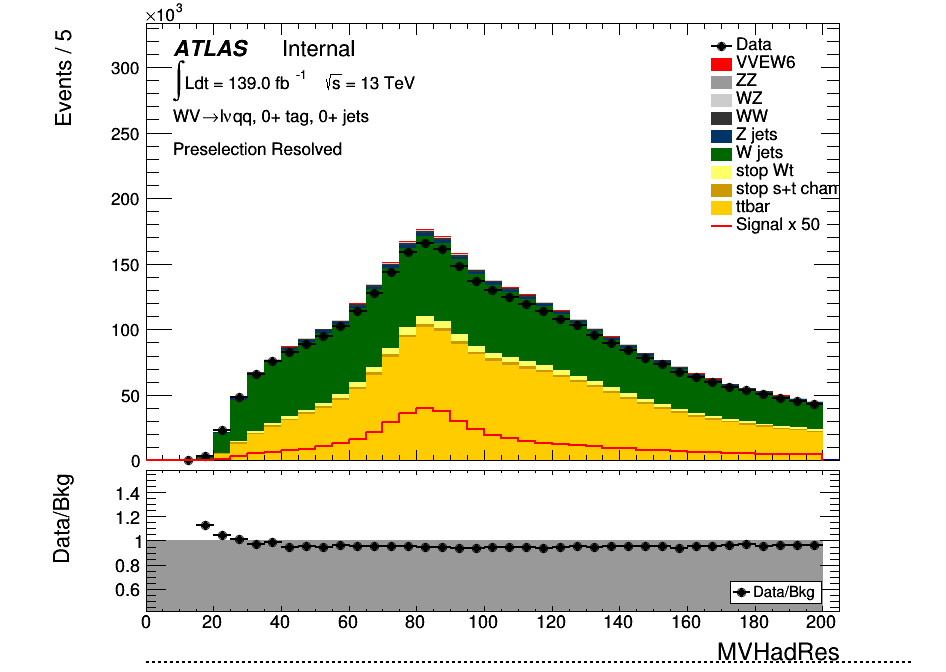
\includegraphics[width=0.3\textwidth]{figures/1lep/CRPlots/C_0ptag0pjet_0ptv_Presel_Resolved_MVHadRes_Lin.png}}
    \subfigure[\emph{\tlep}]{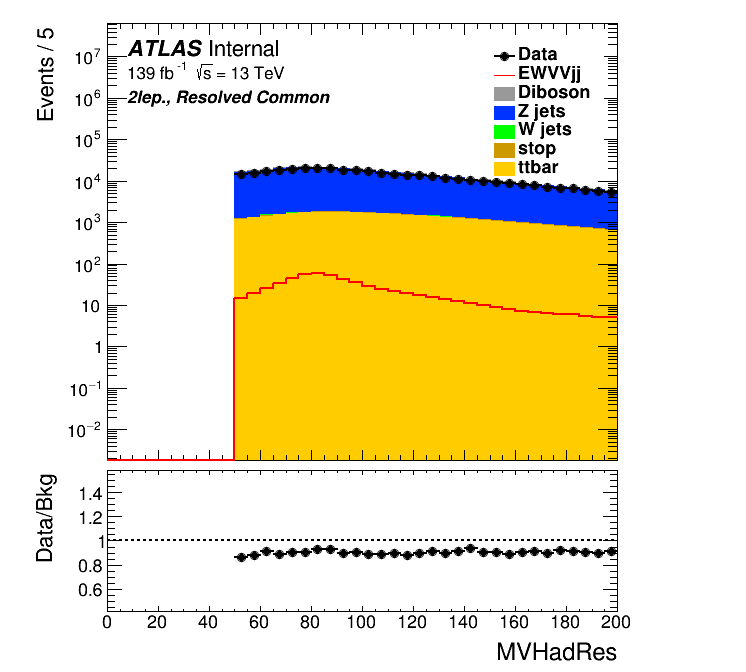
\includegraphics[width=0.3\textwidth]{figures/2lep/dataMC/C_0ptag2pjet_0ptv_ResolvedCommon_MVHadRes_Log.png}}
    \caption{ Mass of reconstructed leading 2 jets in the 1-lepton (left) and 2-lepton channel (right). The plot without mass window cut is shown.} 
    \label{fig:1lep2lepMVHadResSR}
\end{figure}

%\begin{figure}[ht]
%    \begin{center}
%        \subfigure[]{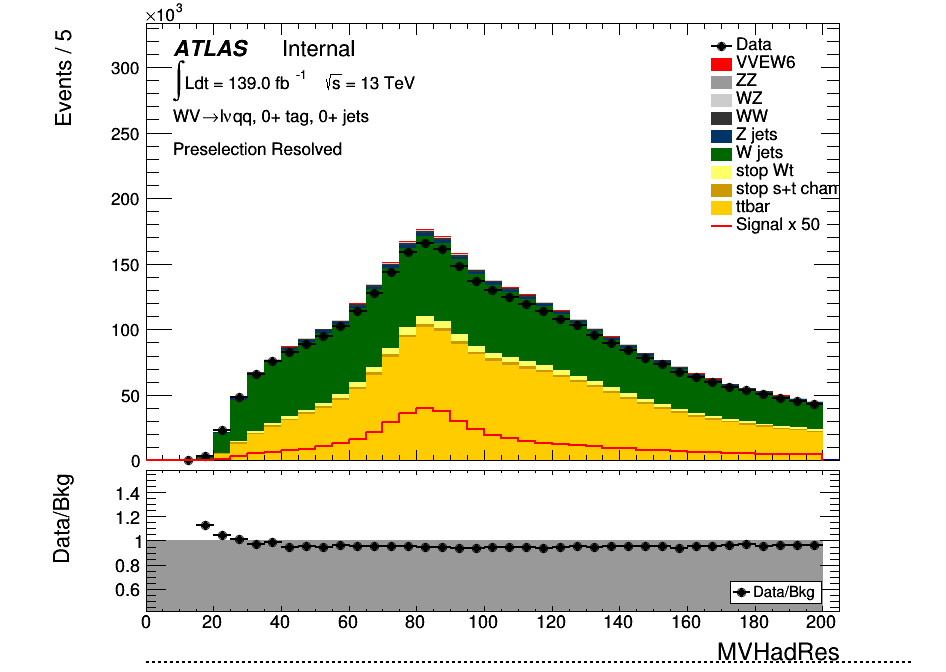
\includegraphics[width=0.3\textwidth]{figures/1lep/CRPlots/C_0ptag0pjet_0ptv_Presel_Resolved_MVHadRes_Lin.png}}
%        \caption{ Mass of reconstructed leading 2 jets in the 1-lepton channel.The plot without mass window cut is shown.}
%    \end{center}
%    \label{fig:1lepMVHadResPresel}
%\end{figure}




\subsubsection{VV system invariant mass for met associated channels}
\label{subsubsec:mVV_reconstruction}


\textbf{Transverse mass $m^T_{ZV}$ in 0-lep}
We use the transverse mass, \mt, reconstructed by \met and the large-R jet for the merged regime while we use \met and the two signal small-R jets in the resolved regime.

\textbf{Reconstruction of $m_{WV}$ in 1-lep} 
%\textcolor{red}{do we use this?? otherwise remove it}

The $WV$ system mass, $m_{WV}$, is reconstructed from the lepton, neutrino and the hadronically-decaying boson candidate (large-R jet or two small-R jets).
The reconstruction of the momentum of the neutrino in the $z$-direction, $p_z$, is obtained by imposing the PDG value of the $W$ boson mass constraint on the lepton and neutrino system, which leads to a quadratic equation. $p_z$ is taken as either the real component of the complex solutions or the one with the smaller absolute value of the two real solutions.

%YIFEI: this is not applied any more 
%In the resolved analysis, the $m_{WV}$ is reconstructed by giving the $W$-($Z$-)mass constraint on the dijet system in the $W \to q\bar{q}$ ($Z \to q\bar{q}$) channel i.e.
%\begin{eqnarray}
%\ptjj^{\textrm{corr}}&=& \ptjj \times \frac{m_{W/Z}}{m_{jj}}; \label{Vmass_constraint1} \\
%m_{jj}^{\textrm{corr}} &=& m_{W/Z}, \label{Vmass_constraint2}
%\end{eqnarray}
%where $m_{jj}$ and $m_{W/Z}$ are the reconstructed invariant mass of the hadronically-decaying $W/Z$ boson and PDG value of the $W/Z$-boson mass, respectively.
%The $m_{WV}$ resolution is improved by ~20\,\% for signal samples and the shape for the background is not so distorted (see details in Ref.~\cite{ATLAS-CONF-2017-051}).
%The background distribution is not so distorted by this operation.
%The improvement is not found in the merged category by imposing $W/Z$-mass constraint on the large-R jet.


%\textbf{Reconstruction of $m_{ZV}$ in 2-lep}
%\textcolor{red}{check if are applying this in 2-lep, I guess NO, if so remove it}

%The $ZV$ system mass, $m_{ZV}$, is reconstructed by the selected two leptons and the hadronically-decaying boson candidate (large-R jet or two small-R jets).
%As with 1-lepton channel, in the resolved category, the $W$- or $Z$-mass constraint on the dijet system in $W\to q\bar{q}$ ($Z\to q\bar{q}$) channel is applied (see Equation~\ref{Vmass_constraint1}--\ref{Vmass_constraint2}).
%Using the same formula, in both merged and resolved categories, 
%the $Z$-mass constraint is applied to dimuon system:
%\begin{eqnarray}
%p_{\textrm{T},\mu\mu}^{\textrm{corr}}&=& p_{\textrm{T},\mumu} \times \frac{m_{Z}}{m_{\mu\mu}}; \\
%m_{\mu\mu}^{\textrm{corr}} &=& m_{Z}.
%\end{eqnarray}
%It compensates the poor muon momentum resolution at the very high-\pt region and  improves the $m_{ZV}$ resolution significantly as described in Ref.~\cite{ATL-COM-PHYS-2016-1494}.
%On the other hand, we didn't find a benefit to give a constraint to dielectron system (better momentum resolution in particular at high-\pt region) so we don't apply it in the electron channel.

\begin{figure}[ht]
    \centering
    \subfigure[merged HP]{\includegraphics[width=0.3\textwidth]{figures/0lep/cutflow/nominal/merged/plots/soverb_individual_SRVBS_HP_MFatJetLow_MFatJet_cutflow.pdf}}
    \subfigure[merged LP]{\includegraphics[width=0.3\textwidth]{figures/0lep/cutflow/nominal/merged/plots/soverb_individual_SRVBS_LP_MFatJetLow_MFatJet_cutflow.pdf}}
    \subfigure[resolved]{\includegraphics[width=0.3\textwidth]{figures/0lep/cutflow/nominal/merged/plots/soverb_individual_SRVBS_Res_MVHadRes_MVHadRes_cutflow.pdf}}
    \caption{0-lepton distribution of the mass of the reconstructed $V_\text{had}$ system. The distributions are shown for the three SR selections. Entering are events passing the respective selection up to the point of the $m(V_\text{had}^\text{reco})$ (where $V_\text{had}^\text{reco}=J^{sig}$ for the merged selection and $V_\text{had}^\text{reco}=(jj)^{sig}$ for the resolved selection) cut which is shown by the vertical line.} 
    \label{fig:0lepMVHad}
\end{figure}

